\chapter[АНАЛИЗ \ ПРОБЛЕМ \ ПЕРЕДАЧИ \ ПОТОКОВОГО ТРАФИКА В ГИБРИДНЫХ СЕТЯХ]{АНАЛИЗ ПРОБЛЕМ ПЕРЕДАЧИ ПОТОКОВОГО ТРАФИКА В ГИБРИДНЫХ СЕТЯХ} \label{chapt1}


\section{Обзор тенденций развития телекоммуникационных технологий} \label{sect1_0}

Объем данных, передаваемый через телекоммуникационные сети, имеет тендецию удваивания ежегодно, что является стимулом исследований для развития сетей следующего поколения.
Сети следующего поколения обычно определяют, как изменение ядра сети с коммутацией каналов на сеть с коммутацией пакетов.
Рассмотрим основные особенности сетей следующего поколения (NGN)\nomenclature{NGN}{Next-Generation Network}.

Телекоммуникационные сети были изначально разработаны для речевого трафика. 
Люди связываются с друг другом, и при этом выделяется целый канал связи от одного телефона к другому. 
Коммутаторы определяют, какой канал должен быть создан и выделяют его на время осуществления сеанса связи.
Этот тип сети обычно называют сеть с коммутацией каналов.

Интернет основан на IP технологии так, что по своей природе является сетью с коммутацией пакетов.
Сети с коммутацией пакетов и сети с коммутацией каналов различны.
В сети с коммутацией каналов, соединение между двумя узлами удерживается на протяжении всего разговора и передача данных другими пользователями через тот же канал не возможна, даже если по линии ничего не передается.
В сети с коммутацией пакетов, нет никакой необходимости, устанавливать постоянное соединение и пакеты могут передаваться между другими пользователями через те же самые каналы связи.

Преимуществом сети с коммутацией каналов является встроенное качество обслуживания (QoS)\nomenclature{QoS}{Quality of Service} так, как коммутатор не будет использовать занятую линию, пока вызов не будет завершен.
Недостатком является то, что это неэффективно, когда нет постоянного потока передаваемых данных.
В противоположность этому, сети с коммутацией пакетов (традиционно) имеют большую пропускную способность.

Одним из путей решения проблемы с сетями с коммутацией пакетов и каналов является запуск двух различных сетей. 
Более старый тип сети с коммутацией каналов только для передачи речи и более современная сеть с коммутацией пакетов для передачи всех других типов данных.
Это довольно дорого так, как в основном необходимо сохранить две отдельные инфраструктуры.
Очевидным решением, которое можно реализовать на основе NGN, является использование только одной сети.


Отличительными чертами NGN является:
обеспечение предоставления неограниченного набора услуг с гибкими возможностями по их управлению,
персонализации и созданию новых услуг за счет унификации сетевых решений, предполагающая реализацию универсальной транспортной сети с распределенной коммуникацией, 
вынесение функций предоставления услуг в оконечные сетевые узлы и интеграция с традиционными сетями связи.

Сети NGN, как правило, строятся по иерархическому принципу, в соответствии с которым можно выделить следующие уровни ее архитектуры (рис. \ref{img:ngn}):

\begin{itemize}
 \item Уровень управления услугами (четвертый уровень), который включает ресурс в виде услуг по доступу пользователей к информации;
 \item Уровень сетевого контроля и управления (третий уровень), основной функцией, которой является управление сетевыми ресурсами, к которым относятся канальные, буферные и информационные;
 \item Транспортный уровень (второй уровень), где реализованы функции транспортной сети, назначением которой является перенос потоков данных (информации) между пользователями;
 \item Уровень доступа (первый уровень) обеспечивает доступ и агрегирование потоков от пользователей различных типов сетей;
 \item Уровень терминального оборудования (нулевой уровень), с помощью которого пользователь использует посредством сети доступа ресурс транспортного уровня.
\end{itemize}

\begin{figure} [!h]
  \center
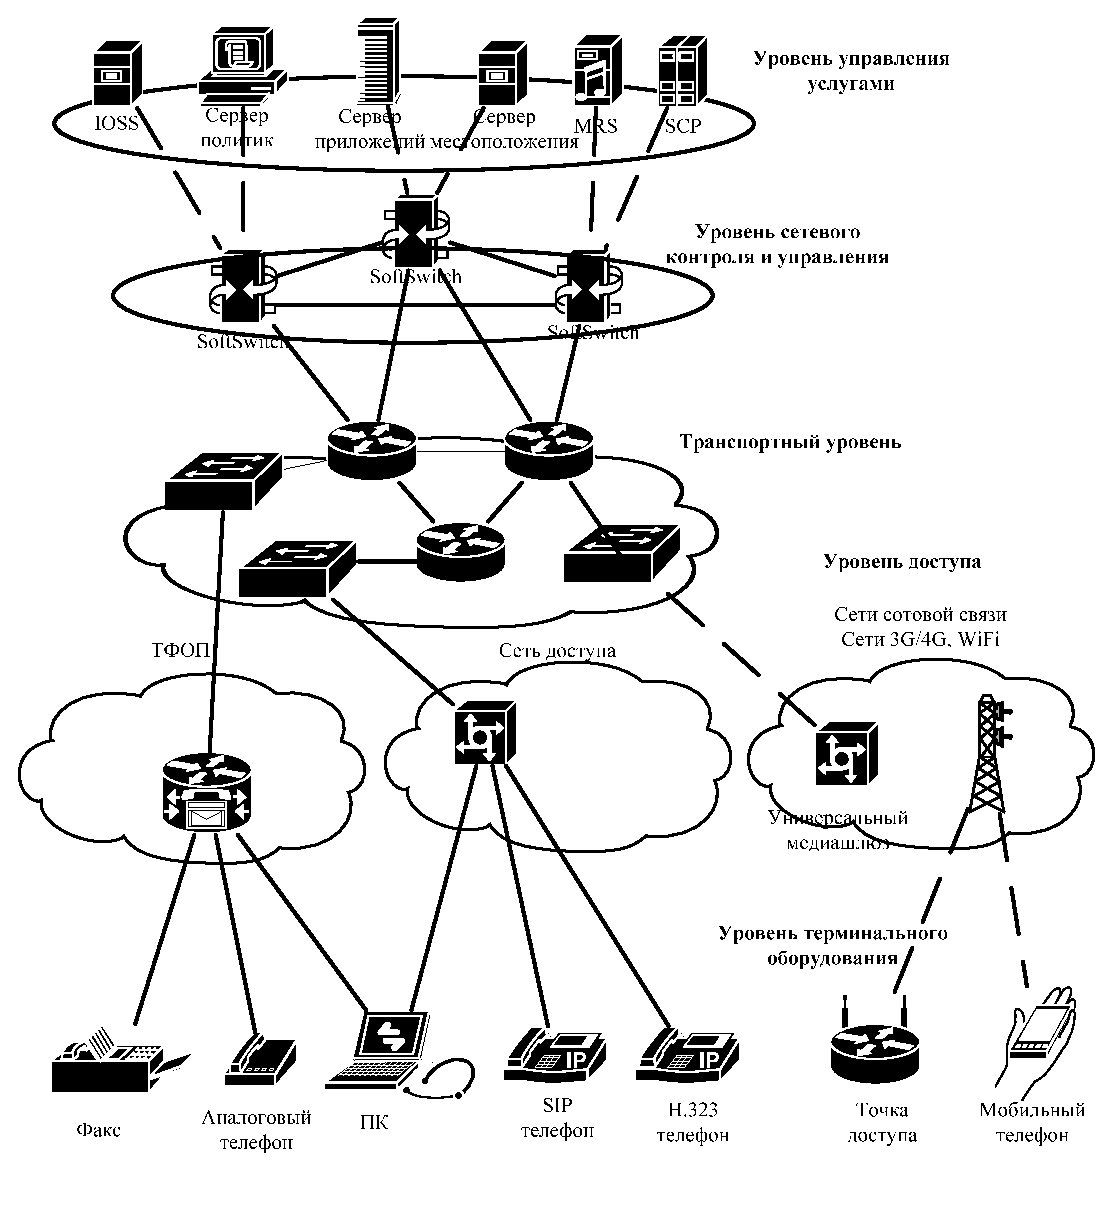
\includegraphics [width=0.95\textwidth] {ngn.eps}
  \caption{Архитектура сети NGN}
  \label{img:ngn}
\end{figure}

\nomenclature{IPTV}{Internet Protocol Television}
\nomenclature{VoIP}{Voice over Internet Protocol}
\nomenclature{SIP}{Session Initiation Protocol}
\nomenclature{IETF}{Internet Engineering Task Force}
\nomenclature{LTE}{Long Term Evolution}
\nomenclature{WiMAX}{Worldwide interoperability for Microwave Access}
\nomenclature{IMS}{IP Multimedia Core Network Subsystem}



Как было сказано ранее, сети следующего поколения являются сетями с коммутацией пакетов и используют протокол IP на сетевом уровне.
В центре сети используется система IP мультимедиа (IMS), которая обеспечивает независимую платформу, через которую сервисы доступа, такие как 4G могут использовать сеть.
Принципиальная идея в том, чтобы предоставить беспрерывную связь: пользователи могут подключаться к сети в любом месте и в любое время.
Ключевым компонентом этого является протокол установки сеансов (SIP).
Он отличается от других протоколов, таких как H.323 тем, что он спроектирован инженерным советом интернета (IETF) специально для IP.
SIP протокол позволил упростить интеграцию таких приложений, как IPTV, VoIP и обмен сообщениями с IP сетями.
Сети четвертого поколения, такие как LTE и WiMAX, работают в направлении принятия NGN. 
Это выражается тем, что:
\begin{enumerate}
 \item LTE и WiMAX были построены с самого начала с использованием в качестве ядра IP сети.
 \item LTE и WiMAX не поддерживают обычных речевых служб.
 \item LTE и WiMAX работают с речевым трафиком также, как и с трафиком данных.
\end{enumerate}


\nomenclature{CDMA}{Code Division Multiple Access}
\nomenclature{HSPA}{High Speed Packet Access}
\nomenclature{WCDMA}{Wideband Code Division Multiple Access}
\nomenclature{GSM}{Global System for Mobile communications}
\nomenclature{EDGE}{Enhanced Data rates for GSM Evolution}
\nomenclature{TD-SCDMA}{Time Division Synchronous Code Division Multiple Access}

\nomenclature{ШПД}{Широкополоный доступ}

Согласно отчету Ericsson \cite{ericsson,ericsson_backgrounder,ericsson_volte} число абонентов мобильной связи во всем мире выросло примерно на 8 процентов в годовом исчислении в 1 квартале 2013 года. Число абонентов мобильной широкополосной связи выросло еще быстрее за этот период в размере 45 процентов в годовом исчислении, достигнув около 1,7 миллиарда. Количество данных, передаваемых каждым устройством, также неуклонно продолжает расти. Около 50 процентов всех проданных мобильных телефонов в 1 квартале 2013 были смартфонами. Все эти факторы привели к удвоению мобильного трафика между 1 кварталом 2012 и 1 кварталом 2013 года. 

В 1 квартале 2013 года общее количество мобильных устройств превысило 6,4 миллиарда. К концу 2018 года ожидается 9,1 миллиард обслуживаемых устройств. 

Глобальное количество обслуживаемых широкополосных устройств достигло в 1 квартал 2013 года 1,7 миллиарда и к концу 2018 года достигнет 7 миллиардов (рис. \ref{img1:mob1}). Основными устройствами широкополосного доступа есть и будут смартфоны. Мобильный широкополосный доступ (ШПД) получит большую долю от общей широкополосной связи на многих рынках, дополняя xDSL\nomenclature{xDSL}{family of technologies Digital Subscriber Line} в определенных сегментах и заменяя его в других. 

Количество обслуживаемых мобильных устройств, таких как мобильные ПК, мобильные роутеры, планшеты, которые используют большой экран, увеличится с 300 млн. в 2012 году до 850 млн. в 2018 году, что превысит число абонентов фиксированной широкополосной связи (рис. \ref{img1:mob2}).
Общее количество смартфонов достигло в 2012 году 1,2 млрд. и, как ожидается, вырастет до 4,5 млрд. в 2018 году. На сегодняшний день основным мобильным устройством является базовый телефон. Проникновение смартфонов будет быстро увеличиваться, в то время как, по оценкам, количество обслуживаемых базовых телефонов останется высоким, медленно снижаясь с 5 млрд. сегодня до 4 млрд. в 2018 году. Это связано с тем, что базовые телефоны будут продолжать находиться в нижнем сегменте продаваемых абонентских устройств.

\pgfplotsset{width=15cm, height=10cm, compat=1.3}
\begin{figure} [!h]
  \center
\begin{tikzpicture}
\pgfkeys{ /pgf/number format/.cd,
        use comma,
        1000 sep={}}
\pgfkeys{/pgfplots/legend pos=north west}
\begin{axis}[
legend cell align=left,
cycle list name=mark list,
xlabel=Год,
ylabel=Количество абонентов/линий (млн)
]

\addplot coordinates
{(2009,4200) (2010,4850) (2011,5500) (2012,6000) (2013,6500) (2014,7000) (2015,7500) (2016,8000) (2017,8500) (2018,9000)};

\addplot coordinates
{(2009,300) (2010,600) (2011,1000) (2012,1500) (2013,2100) (2014,3000) (2015,3700) (2016,4800) (2017,5800) (2018,7000)};

\addplot coordinates
{(2009,500) (2010,525) (2011,550) (2012,575) (2013,600) (2014,625) (2015,650) (2016,675) (2017,700) (2018,725)};

\addplot coordinates
{(2009,50) (2010,140) (2011,230) (2012,320) (2013,410) (2014,500) (2015,590) (2016,680) (2017,770) (2018,860)};
\legend{Мобильные абоненты, Мобильные широкополосные линии, Проводные широкополосные линии, Мобильные ПК/планшеты/мобильные роутеры}
\end{axis}
\end{tikzpicture}
\caption{Стационарные и мобильные обслуживаемые устройства, 2009-2018 \cite{ericsson}}
  \label{img1:mob1}
\end{figure}


\pgfplotsset{width=15cm, height=10cm, compat=1.3}
\begin{figure} [!h]
  \center
\begin{tikzpicture}
\pgfkeys{ /pgf/number format/.cd,
        use comma,
        1000 sep={}}
\pgfkeys{/pgfplots/legend pos=north west}



\begin{axis}[stack plots=y,/tikz/ybar,
legend cell align=left,
cycle list name=mark list,
xlabel=Год,
ylabel=Количество абонентов (млн)
]
\addplot coordinates
{(2010,4466) (2011,4711) (2012,4741) (2013,4639) (2014,4483) (2015,4289) (2016,4099) (2017,3926) (2018,3763)};
\addplot coordinates
{(2010,522) (2011,836) (2012,1247) (2013,1781) (2014,2363) (2015,2944) (2016,3504) (2017,4017) (2018,4493)};
\addplot coordinates
{(2010,166) (2011,238) (2012,308) (2013,386) (2014,467) (2015,554) (2016,647) (2017,745) (2018,846)};

\legend{Функциональный/Базовый телефон, Смартфон, Мобильный ПК/Маршрутизатор/Планшет}
\end{axis}
\end{tikzpicture}
\caption{Прогноз развития беспроводных сетей по устройствам \cite{ericsson}}
  \label{img1:mob2}
\end{figure}




На рис. \ref{img1:mob3} иллюстрирован отчет по количеству обслуживаемых мобильных устройств различными технологиями: LTE, WCDMA/HSPA,\\ GSM/EDGE, TD-SCDMA, CDMA и другими. Технология LTE, которая развернута и представлена во всех регионах, в 2018 году составит 2 млрд. устройств. Эти устройства будут представлять лидирующую долю от общего количества устройств. Быстрый переход на более совершенные технологии в развитых странах, означает, что мировое количество абонентов GSM/EDGE будет снижаться после 2012-2013 годов. Глобально, GSM/EDGE будет продолжать играть ведущую роль с точки зрения числа абонентов до последних лет прогнозного периода. Это связано с тем, что новые менее обеспеченные пользователи, вероятно, будут использовать самые дешевые мобильные устройства и технологии мобильной связи. Кроме этого требуется время для обновления установленной базы мобильных устройств.


\pgfplotsset{width=15cm, height=10cm, compat=1.3}
\begin{figure} [!h]
  \center
\begin{tikzpicture}
\pgfkeys{ /pgf/number format/.cd,
        use comma,
        1000 sep={}}
\pgfkeys{/pgfplots/legend pos=north west}
\begin{axis}[stack plots=y,/tikz/ybar,
legend cell align=left,
cycle list name=mark list,
xlabel=Год,
ylabel=Количество абонентов (млн)
]
\addplot coordinates
{(2010,64) (2011,54) (2012,37) (2013,34) (2014,35) (2015,35) (2016,35) (2017,29) (2018,23)};
\addplot coordinates
{(2010,497) (2011,532) (2012,545) (2013,537) (2014,525) (2015,514) (2016,503) (2017,485) (2018,473)};
\addplot coordinates
{(2010,21) (2011,51) (2012,94) (2013,149) (2014,199) (2015,229) (2016,231) (2017,223) (2018,201)};
\addplot coordinates
{(2010,3904) (2011,4182) (2012,4311) (2013,4263) (2014,4060) (2015,3717) (2016,3240) (2017,2696) (2018,2117)};
\addplot coordinates
{(2010,668) (2011,956) (2012,1245) (2013,1648) (2014,2148) (2015,2710) (2016,3321) (2017,3874) (2018,4336)};
\addplot coordinates
{(2010,0) (2011,9) (2012,64) (2013,176) (2014,346) (2015,583) (2016,920) (2017,1381) (2018,1953)};

\legend{Other Technology, CDMA, TD-SCDMA, GSM/EDGE, WCDMA/HSPA, LTE}
\end{axis}
\end{tikzpicture}
\caption{Прогноз развития беспроводных сетей по технологиям \cite{ericsson}}
  \label{img1:mob3}
\end{figure}


На рис. \ref{img1:mob4} изображена устойчивая тенденция роста трафика данных с некоторыми сезонными колебаниями. Это показывает, что мобильные данные абонентов сильно вырастут. Ведущую роль в увеличении общего количества трафика данных сыграло непрерывное увеличение среднего объема данных, передаваемое и принимаемое с каждого устройства.





\pgfplotsset{
    /pgfplots/area legend/.style={%
        /pgfplots/legend image code/.code={%
            \fill[##1] (0cm,-0.1cm) rectangle (0.6cm,0.1cm);
        }%
    },
}



\usetikzlibrary{patterns}

\begin{figure} [!h]
  \center
%\includegraphics[width=0.95\textwidth]{ericsson/mob5.png}
\begin{tikzpicture}
\begin{axis}[
legend cell align=left,
cycle list name=linestyles*,
area legend,
axis x line=bottom,
axis y line=left,
legend style={at={(0.03,0.97)},anchor=north west},
xlabel=Год,
ylabel=Общий трафик (Петабайт),
ymin=0,
ybar,
bar width=5pt,
Axis Style,
    xtick={
        2007, 2007.25, 2007.5, 2007.75,
        2008, 2008.25, 2008.5, 2008.75,
        2009, 2009.25, 2009.5, 2009.75,
        2010, 2010.25, 2010.5, 2010.75,
        2011, 2011.25, 2011.5, 2011.75,
        2012, 2012.25, 2012.5, 2012.75,
        2013, 2013.25, 2013.5, 2013.75
    },
    xticklabels={
        $\tiny \begin{array}{c}Q1 \\ 2007\end{array}$, $\tiny \begin{array}{c}Q2 \end{array}$, $\tiny \begin{array}{c}Q3\end{array}$, $\tiny \begin{array}{c}Q4\end{array}$,
        $\tiny \begin{array}{c}Q1 \\ 2008\end{array}$, $\tiny \begin{array}{c}Q2\end{array}$, $\tiny \begin{array}{c}Q3\end{array}$, $\tiny \begin{array}{c}Q4\end{array}$,
        $\tiny \begin{array}{c}Q1 \\ 2009\end{array}$, $\tiny \begin{array}{c}Q2\end{array}$, $\tiny \begin{array}{c}Q3\end{array}$, $\tiny \begin{array}{c}Q4\end{array}$,
        $\tiny \begin{array}{c}Q1 \\ 2010\end{array}$, $\tiny \begin{array}{c}Q2\end{array}$, $\tiny \begin{array}{c}Q3\end{array}$, $\tiny \begin{array}{c}Q4\end{array}$,
        $\tiny \begin{array}{c}Q1 \\ 2011\end{array}$, $\tiny \begin{array}{c}Q2\end{array}$, $\tiny \begin{array}{c}Q3\end{array}$, $\tiny \begin{array}{c}Q4\end{array}$,
        $\tiny \begin{array}{c}Q1 \\ 2012\end{array}$, $\tiny \begin{array}{c}Q2\end{array}$, $\tiny \begin{array}{c}Q3\end{array}$, $\tiny \begin{array}{c}Q4\end{array}$,
        $\tiny \begin{array}{c}Q1 \\ 2013\end{array}$, $\tiny \begin{array}{c}Q2\end{array}$, $\tiny \begin{array}{c}Q3\end{array}$, $\tiny \begin{array}{c}Q4\end{array}$
    }
]
\addplot [pattern color=red!50, draw=black, pattern=north west lines] coordinates
{(2007,70) (2007.25,75) (2007.5,80) (2007.75,85) (2008,90) (2008.25,100) (2008.5,110) (2008.75,120) (2009,130) (2009.25,140) (2009.5,145) (2009.75,150) (2010,155) (2010.25,160) (2010.5,160) (2010.75,160) (2011,160) (2011.25,160) (2011.5,160) (2011.75,160) (2012,160) (2012.25,160) (2012.5,160) (2012.75,160) (2013,160) (2013.25,0)}
\closedcycle;

\addplot [pattern color=blue!50, draw=black, pattern=north east lines] coordinates
{(2007,3) (2007.25,5) (2007.5,8) (2007.75,10) (2008,13) (2008.25,15) (2008.5,20) (2008.75,30) (2009,50) (2009.25,80) (2009.5,120) (2009.75,160) (2010,180) (2010.25,220) (2010.5,250) (2010.75,320) (2011,390) (2011.25,400) (2011.5,480) (2011.75,560) (2012,760) (2012.25,840) (2012.5,1000) (2012.75,1280) (2013,1520) (2013.25,0)}
\closedcycle;

\legend{Речь, Данные}
\end{axis}



\end{tikzpicture}
  \caption{Глобальный общий трафик передачи речи и данных в мобильных сетях, 2007-2013 \cite{ericsson}}
  \label{img1:mob4}
\end{figure}



Рост числа абонентов в широкополосной мобильной связи, является мощным стимулом роста для мобильного трафика. С увеличением числа пользователей, увеличивается количество устройств подключенных к сети, таких как смартфоны, планшеты, мобильные ПК, мобильные роутеры, электронные книги и камеры.  Самым быстрорастущим сегментом в мобильном трафике является видео. Увеличение использования контента приводит в постоянный рост количество доступного контента, а так же к лучшим сетевым скоростям, которые приходят с развитием HSPA и LTE. Рост размеров экранов устройств и разрешения экранов, также будут драйвером увеличения мобильного трафика, так как они позволят смотреть видео высокой четкости, а в дальнейшем и сверхвысокой. 

Сервисы с потоковым видео так же имеют высокую популярность. Люди используют эти сервисы на всех типах устройств. 
Так же видеоконференции при использовании мобильных устройств, будут стимулировать рост видео трафика в мобильных сетях. 
Сегодня передача видео контента составляет крупнейший сегмент трафика данных в мобильных сетях, и, как ожидается, будет расти примерно на 60 процентов в год вплоть до конца 2018 года, на этот момент, по прогнозам, объем видео трафика составит около половины от общего глобального трафика (рис. \ref{img1:mob7}).

Потоковая музыка приобретает все большую популярность и аудио как ожидается, будет расти с годовым темпом роста около 50 процентов. 
Существует высокая степень неопределенности в прогнозе на аудио трафик на данном этапе, так как он очень сильно зависит от того, как сервисы потоковой музыки будут развиваться в ближайшие годы.
Просмотр веб-страниц и социальных сетей будет каждый составлять около 10 процентов от общего объема трафика данных в 2018 году.
Приход новых типов устройств или информационного контента способного быстро изменить трафик, в настоящее время, не считается значительным. Кроме того, будет широкая вариация между сетями с различными профилями устройств, например, некоторые из них будут с доминированием PC в то время как другие будут способствовать использованию смартфонов. Трафик также будет меняться между рынками из-за различий в доступности контента и прав. 

\definecolor{RYB3}{RGB}{190, 186, 218}
\definecolor{RYB1}{RGB}{141, 211, 199}
\begin{figure} [!h]
  \center
%\includegraphics[width=0.95\textwidth]{ericsson/mob5.png}
\begin{tikzpicture}

\pgfkeys{ /pgf/number format/.cd,
        use comma,
        1000 sep={}}

\begin{axis}[
legend cell align=left,
stack plots=y,
%area style,
enlarge x limits=false,
area legend,
axis x line=bottom,
axis y line=left,
domain=0:1,
legend style={at={(0.03,0.97)},anchor=north west},
xlabel=Год,
ylabel=Общий месячный трафик ($10^{18}$ байт)
]
\addplot[pattern color=blue!50, draw=black, pattern=vertical lines] coordinates
{(2010,0.05) (2012,0.06) (2013,0.1) (2014,0.15) (2015,0.2) (2016,0.3) (2017,0.4) (2018,0.5)}
\closedcycle;

\addplot[pattern color=red!50, draw=black, pattern=horizontal lines] coordinates
{(2010,0.05) (2012,0.4) (2013,0.9) (2014,1.5) (2015,2.3) (2016,3.5) (2017,5.2) (2018,7)}
\closedcycle;

\addplot[pattern color=blue!50, draw=black, pattern=north west lines] coordinates
{(2010,0.03) (2012,0.05) (2013,0.07) (2014,0.1) (2015,0.15) (2016,0.2) (2017,0.25) (2018,0.3)}
\closedcycle;

\addplot[pattern color=green!50, draw=black, pattern=fivepointed stars] coordinates
{(2010,0.05) (2012,0.12) (2013,0.2) (2014,0.4) (2015,0.6) (2016,0.9) (2017,1.1) (2018,1.6)}
\closedcycle;

\addplot[pattern color=orange!100, draw=black, pattern=dots] coordinates
{(2010,0.04) (2012,0.1) (2013,0.15) (2014,0.2) (2015,0.4) (2016,0.6) (2017,0.9) (2018,1.1)}
\closedcycle;

\addplot[pattern color=RYB1!100, draw=black, pattern=grid] coordinates
{(2010,0.04) (2012,0.1) (2013,0.17) (2014,0.23) (2015,0.3) (2016,0.4) (2017,0.5) (2018,0.7)}
\closedcycle;

\addplot[pattern color=RYB3!100, draw=black, pattern=sixpointed stars] coordinates
{(2010,0.04) (2012,0.1) (2013,0.17) (2014,0.25) (2015,0.35) (2016,0.5) (2017,0.7) (2018,0.9)}
\closedcycle;

\addplot[pattern color=blue!50, draw=black, pattern=north east lines] coordinates
{(2010,0.05) (2012,0.1) (2013,0.2) (2014,0.5) (2015,1) (2016,1.4) (2017,1.7) (2018,2)}
\closedcycle;

\legend{Файлы в общем доступе, Видео, Аудио, Веб сайты, Социальные сети, Скачивание и обновление ПО, Шифрованный трафик, Другое}
\end{axis}
\end{tikzpicture}
  \caption{Глобальный трафик, разбитый по приложениям, 2010-2018 \cite{ericsson}}
  \label{img1:mob7}
\end{figure}



Когда пользователь меняет свой телефон на смартфон, он все равно продолжает пользоваться речевыми и текстовыми сообщениями. Пользователи склонны к развитию привычки использования приложения в течении некоторого времени после того как они открыли новое приложение или сервис. Рекомендации пользователей, семьи, рекламы и магазинов для новых и трендовых приложений играют значительную роль. 

Со временем, пользователи, как правило, используют более современные услуги, которые ставят более высокие требования к возможностям устройства. Сегодня пользователи смартфонов, которые подключаются к сервисам с музыкой и потоковым видео уже потребляют больше, чем 2 Гб трафика в месяц в среднем. Это в четыре раза больше потребления среднего пользователя со смартфоном. Во многих магазинах, легальные потоковые сервисы для музыки и для видео набирают популярность. При достаточном контенте и правильном уровне цен эти услуги демонстрируют высокие темпы популяризации.

Прогнозы для каждой категории мобильных данных показывают значительный рост до 2018 года. 
Наибольший прирост ожидается от видео трафика, и, по оценкам, составит около половины всего мобильного трафика данных к концу прогнозируемого периода. 
Видео трафик, скорее всего, представит большую часть всего мобильного трафика данных к 2018 году.



%Вследствие всего выше перечисленного, потоковый трафик набирает все большую популярность и обеспечение 















\section{Анализ предпосылок внедрения услуг передачи речи и видео в беспроводных сетях LTE} \label{sect1_4}



Мобильная связь стандарта LTE оптимизирована для передачи данных и реализована в виде коммутации пакетов через IP. LTE не включает в себя домен с коммутацией каналов, который в настоящее время используется для предоставления услуг передачи речи и SMS услуг. Спрос на услуги мобильного широкополосного доступа растет, и операторы запускают высокоскоростные сети на основе технологии LTE. Тем не менее, услуги передачи речи и SMS услуги приносят около 70\% от общей выручки операторов и ясно, что эта функциональность должна быть реализована в сетях LTE.

С передачей речи поверх LTE (GSMA VoLTE IR.92 спецификация, основанная на глобальных 3GPP стандартах) абоненты получают возможность речевой и видео связи и другие услуги для LTE смартфонов \cite{IMS,ir92,ir94}.

Для реализации услуг передачи речи поверх сети LTE, необходимо чтобы IMS  (IP Multimedia System) ядро сети предоставляло сервис телефонии поверх IP. MMTel  (Multi Media Telephony, разработанная в IMS ядре) является решением, которое предоставляет услуги телефонии (включая видео связь, чат и другое) как в LTE, так и в фиксированной сети. LTE сеть радио доступа и EPC также должно поддерживать VoLTE, которое может быть достигнуто обновлением программного обеспечения.

Операторы могут использовать то же самое ядро сетевой инфраструктуры IMS в VoLTE для развития мобильной и фиксированной конвергенции между любыми устройствами.
Пользователи будут иметь возможность использовать предоставляемую оператором высококачественную речевую и видео связь и другие услуги связи на LTE смартфонах и других устройствах.

Эти услуги используют обычный номер мобильного телефона (MSISDN, Mobile Subscriber Integrated Services Digital Network-Number), а VoLTE приносит функции мобильного оператора в мобильную широкополосную сеть, основанную на IP. С помощью VoLTE услуги передачи речи могут быть использованы одновременно на LTE устройства.








Мобильный широкополосный доступ создал целый мир возможностей и открыл новые источники дохода для операторов. Возможности часто сочетаются с проблемами. Решающий вопрос состоит в том, чтобы воспользоваться возможностями широкополосного доступа и в тоже время сохранить и увеличить доходы от услуг связи, таких как передача речи и SMS. Сети LTE могут предоставлять широкополосный доступ и услуги связи с большими возможностями и с меньшей задержкой.  

\begin{figure} [h]
  \center
\includegraphics [width=0.95\textwidth] {ericsson/volte1.png}
  \caption{Общий сетевой обзор решения VoLTE (IMS, EPC, LTE), включая поддержку устаревших сетей, когда пользователь находится за пределами покрытия LTE \cite{ericsson_backgrounder}}
  \label{img:volte1}
\end{figure}

Некоторые ОТТ (Over the Top) решения, такие как Skype, часто предустановленные на смартфоны, получили широкое распространение. Термин OTT означает доставку видео и аудио сигнала на приставку (компьютер, мобильный телефон) пользователя по сети Интернет без прямого контакта с оператором связи в отличие от услуг VoIP и IPTV, которые предоставляются через управляемую оператором сеть с гарантированным QoS. Тем не менее, ОТТ решения не могут полностью удовлетворить пользователей, так как предоставляются без гарантированного QoS, нет поддержки хэндовера в сеть с коммутацией каналов, нет широкого взаимодействия услуг между различными службами OTT и устройствами, нет поддержки вызова чрезвычайных служб, имеют проблемы с безопасностью. Следовательно, использование сервисов OTT клиентом напрямую зависит от покрытия мобильной широкополосной связи и готовностью абонентами использовать сервис, который испытывает недостаток в качестве, безопасности и гибкости. 

Операторы уже сейчас могут начать глобальное развертывание коммерческих решений речевой и видео связи поверх LTE - еще до того, когда LTE сеть будет полностью развернута.

LTE и EPC архитектуры не включают поддержку коммутации речевой и видео связи. 
Перед началом использования LTE в телефонах, это ограничение должно быть решено. На данный момент существует два решения этой проблемы \cite{ericsson_backgrounder}: CS fallback (CSFB) и IMS/VoLTE. CSFB подходит для использования, когда LTE покрытие является неоднородным (как правило, на ранних этапах развертывания LTE), а IMS/VoLTE может быть реализована, когда покрытие практически однородно (как правило, когда сеть LTE уже в более зрелом состоянии).






\section{Анализ требований QoS для предоставления сервисов реального времени } \label{sect_qos}

Основными факторами,  влияющими на качество передачи речи в IP  сетях,  являются задержка передачи и процент потери пакетов \cite{G114}.
На рис. \ref{img1:qos_dd} показаны контуры качества передачи речи (удовлетворенности пользователя) для кодека G.711 с включенной функцией скрытия потерь пакетов (PLC).





Наибольший вклад в задержку и потери пакетов вносит не оптимальный буфер компенсации джиттера. 

На рис. \ref{img1:qos_dd} видно, что качество передачи
речи уменьшается с увеличением задержки и
процента потери пакетов. Необходимо определить составляющие, которые вносят
наибольший вклад в задержку и потерю пакетов.
Составляющие задержки при передаче речи средствами VoIP:
\begin{enumerate}
 \item Аналого-цифровое и цифро-аналоговое преобразование сигнала.
 \item Кодирование/компрессия и декодирование/декомпрессия.
 \item Упаковка блока данных и распаковка блока данных стека протоколов TCP/IP.
 \item Буфер компенсации джиттера.
\end{enumerate}


\pgfplotsset{width=15cm, height=10cm, compat=1.3}
\begin{figure} [h]
  \center
\begin{tikzpicture}
\pgfkeys{ /pgf/number format/.cd,
        use comma,
        1000 sep={}}
\pgfkeys{/pgfplots/legend pos=north west}
\begin{axis}[
legend cell align=left,
cycle list name=mark list,
xlabel=Задержка (мс),
ylabel=Пакетные потери (\%),
xmin=0,
xmax=500,
ymax=20,
ymin=0,
]
\node
	at (50,6) {\scriptsize Очень довольны};
\node
	at (70,25) {\scriptsize Пользователи довольны};
\node
	at (100,60) {\scriptsize Некоторые пользователи довольны};
\node
	at (100,100) {\scriptsize Многие пользователи не довольны};
\node
	at (105,160) {\scriptsize Почти все пользователи не довольны};
\node
	at (400,160) {\scriptsize Не рекомендуется};
\addplot[mark=none] coordinates
{(0,1.1) (159,1.1) (205,0)};
\addplot[mark=none] coordinates
{(0,4.1) (159,4.1) (175,3.9) (285,0)};
\addplot[mark=none] coordinates
{(0,8.1) (175,8.1) (265,4.2) (390,0)};
\addplot[mark=none] coordinates
{(0,13.5) (175,13.5) (500,1)};
\addplot[mark=none] coordinates
{(0,20) (200,20) (500,4)};

\end{axis}
\end{tikzpicture}
\caption{Контуры качества передачи речи G711 c PLC}
  \label{img1:qos_dd}
\end{figure}


Для большинства оконечных устройств, работающих с VoIP, потерями на аналого-цифровое и цифро-аналоговое преобразование, 
декодирование/декомпрессию и формирование стека протоколов TCP/IP можно пренебречь. 
Средняя величина задержки, вносимой каждой из составляющих VoIP \cite{G114,Y1541}, представлена в табл. \ref{tb:dl} \cite{rokovoy}.



В соответствии с рекомендациями \cite{G114} максимальная задержка при передаче речи в одну сторону не должна превышать 150 мс.
Таким образом, в зависимости от параметров сети, до 40\% допустимой задержки может составлять задержка в буфере компенсации джиттера.
Буфер компенсации джиттера компенсирует отклонения значений задержки от среднего значения. Прибывающие пакеты на приемной стороне
воспроизводятся не сразу, а с определенной задержкой. Чем больше джиттер, тем больше размер буфера требуется для компенсации изменений задержки, иначе часть пакетов будет отброшена, если они придут позже времени воспроизведения. 
При максимальном размере буфера появляется возможность свести количество отбрасываемых пакетов к минимуму, но при этом увеличивается время задержки. 
При минимальном размере буфера время задержки уменьшается, но при этом увеличивается количество отбрасываемых пакетов.

{%
\newcommand{\mc}[3]{\multicolumn{#1}{#2}{#3}}
\begin{table} [hbt]
  \parbox{15cm}{\caption{Типы и параметры буфера компенсации джиттера}\label{tb:dl}}
\begin{center}
\begin{tabular}[t]{| p{12cm} | p{3cm} |}\hline \hline
\mc{1}{|c|}{Наименование} & \mc{1}{c|}{Вносимая задержка}\\ \hline \hline
Оптический кабель & 5 мкс/км\\ \hline
Система наземной мобильной связи & 80-110 мс\\ \hline 
Кодек G.729 для 20 мс блоков & 25 мс\\ \hline
Кодек GSM для 20 мс блоков & 20 мс\\ \hline
Сетевое оборудование (L3), суммарное время нахождения в очереди и обработка & 2-10 мс на узел\\ \hline
Буфер компенсации джиттера & 20-60 мс\\ \hline
\end{tabular}
\end{center}
\end{table}

}%


Следовательно, размер буфера должен меняться во времени по алгоритму, учитывающему текущее состояние сети. 
И чем быстрее метод реагирует на изменения состояния сети, тем выше качество предоставляемого потокового сервиса на приемной стороне. 
Поэтому возникает задача: разработать метод адаптивного управления буфером компенсации джиттера.


\section{Анализ работы буфера компенсации джиттера и рабочих характеристик применительно к передаче потокового трафика через IP-сети} \label{sect3_2}

Буфер воспроизведения в приемнике удерживает каждый принятый пакет на величину времени буфера, в котором компенсируется джиттер без чрезмерной задержки воспроизведения. Если межпакетная задержка будет превышать буферное время, буфер будет истощаться, и декодеру не будет хватать пакетов, чтобы воспроизводить речь. Это приводит к неравномерности воспроизведения речи. 
Согласно рекомендации ITU G.1020 \cite{G1020} пакеты, прибывающие к получателю, обрабатываются согласно процессу, изображенному на рис. \ref{img3:algh_pack}.

\begin{figure} [h]
  \center
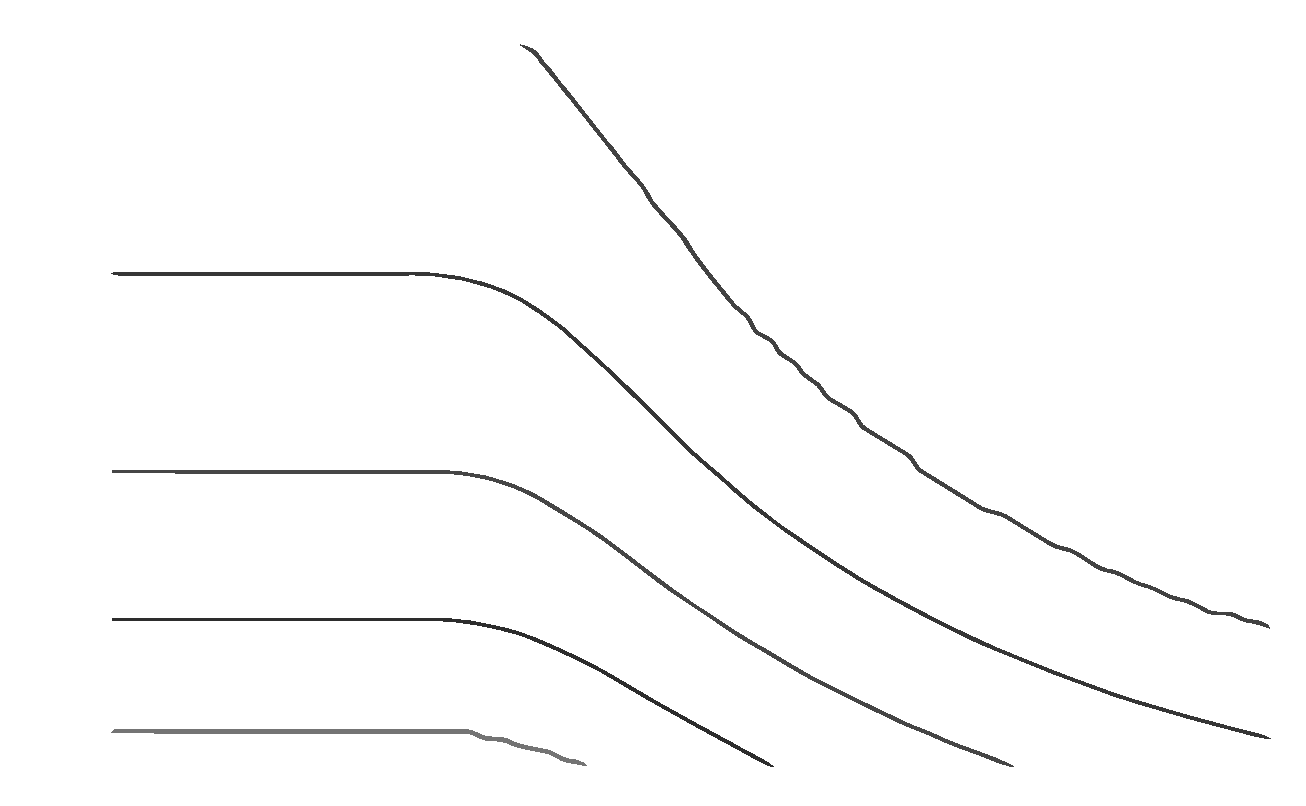
\includegraphics[width=0.95\textwidth]{3chapter/3.eps}
  \caption{Алгоритм обработки сетевых пакетов}
  \label{img3:algh_pack}
\end{figure}

Прибывающие пакеты обрабатываются по мере их продвижения по стеку протокола. 
Показано, что некоторые характеристики, такие как ошибки и джиттер преобразуются в общие потери и общие ошибки.
На рис. \ref{img3:algh_pack} показан компромисс между задержкой и потерями, представленные в виде порога в диапазоне изменения задержки, основанном на размере буфера для сглаживания джиттера. 
Пакеты с задержкой находящейся в белой зоне будут приняты, тогда как пакеты с задержкой находящейся в черной зоне будут отброшены. 
Ясно, что чем больше задержка, тем больше пакетов прибудет до их времени воспроизведения и тем лучше будет компенсация джиттера. 
В тоже время, длительные задержки нежелательны, так как они ухудшают интерактивность человеческого общения. 
Отметим, что человеческое ухо терпимо относится к максимальным задержкам от 150 до 400 миллисекунд \cite{Moon}. 

Различные схемы кодирования также могут иметь различные допуски к потерям. 
Как следствие, хороший алгоритм компенсации джиттера основан на компромиссе между задержкой воспроизведения и потерями пакетов.
Рассмотрим изменение процесса потерь во время взаимодействие пакетов с буфером компенсации джиттера. 
В зависимости от критерия, определяющего решение принимать или отбрасывать каждый конкретный пакет из потока, в результате может полностью измениться распределение общих потерь и общей задержки. 
Например, если случайные битовые ошибки вызывают ошибки в контрольной сумме UDP, то потери пакетов будут иметь случайное распределение, по мере того как они поступают на прикладной уровень. 
Но, если несколько последовательных пакетов испытывают чрезмерные задержки, то дополнительные отбрасывания, вызванные ограничениями буфера компенсации джиттера, 
сделают общее распределение потерь еще и прерывистым.
Существуют обстоятельства, при которых порядок следования пакетов может изменяться во время их прохождения через сеть. 

При определенных условиях некоторые буферы компенсации джиттера неспособны восстановить порядок следования переупорядоченных пакетов и, в этом случае, они обозначаются как отброшенные пакеты.
Также рассмотрим влияние буфера компенсации джиттера на процесс задержки. 
На рис. \ref{img3:delNode} показаны основные элементы тракта передачи речи, которые вносят вклад в речевую задержку. 
Задержка сети переменна и для компенсации джиттера и восстановления допустимого интервала между пакетами используют буфер компенсации джиттера. 
Заметим, что пакеты с минимальной задержкой на стороне отправителя и сети, проводят максимальное время в буфере компенсации джиттера; и наоборот, пакеты, 
которые задерживаются дольше минимального времени, проводят затем в данном буфере меньшее время. 
Кроме того, существует еще, и некоторое минимальное количество времени, которое каждый пакет должен проводить в буфере на стороне получателя, которое может быть столь же велико, как и целый пакет.

\begin{figure} [h]
  \center
\includegraphics[width=0.95\textwidth]{3chapter/2.eps}
  \caption{Задержка в пакетных сетях и сетевых элементах}
  \label{img3:delNode}
\end{figure}

Правильное значение задержки буфера для объединения с другими задержками зависит от наличия описательной статистики. 
Например, среднюю задержку в сети следует суммировать со средним временем использования буфера компенсации джиттера, чтобы получить общую среднюю задержку. 
Этот метод предусматривает адаптацию буфера, требуя знания только среднего времени пребывания всех пакетов в очереди в оцениваемом временном интервале. 
С другой стороны, если известна только минимальная задержка в сети, то ее следует суммировать с максимальным временем использования буфера компенсации джиттера, чтобы дать общую задержку.
Далее рассмотрим инициализацию буфера компенсации джиттера фиксированного размера. 
Если первый прибывающий пакет имеет минимальную задержку передачи, то получатель будет сохранять этот пакет в буфере все необходимое время, и размер буферизации будет равен ожидаемому. 
К счастью, многие пакеты прибывают за время, равное или близкое к минимальному времени передачи, поэтому этот случай весьма правдоподобен. 
С другой стороны, если первый пакет имеет довольно большую задержку, 
то для размещения ранее принятых пакетов со временем передачи, равным или близким к минимальному времени передачи, 
потребуется больше буферного пространства, а буфер для сглаживания фазового дрожания будет вносить в общий расчет задержку, превышающую ожидаемую.

\section{Систематизация типов, параметров и моделей буферов компенсации джиттера} \label{sect3_3}

Существуют два основных типа буферов компенсации джиттера – фиксированной длины и адаптивной длины. Буферы компенсации джиттера, согласно рекомендации \cite{G1020}, могут быть построены с использованием разных способов, приведенных в табл. \ref{TypeBuff}.

Более подробно рассмотрим параметры построения алгоритма адаптивного буфера компенсации джиттера по методу подстройки задержки воспроизведения, такие как алгоритмы выполняющие коррекцию синхронно и алгоритмы выполняющие коррекцию в промежутках между речевыми потоками. 
В схеме с синхронизированной подстройкой задержки воспроизведения (рис. \ref{img3:manageDelay} a) время воспроизведения всех последующих пакетов растягивается всякий раз, когда пакет чрезмерно задерживается в сети. 
Во втором случае, показанном на рис. \ref{img3:manageDelay} б, производится корректировка первого пакета речевого потока, а все остальные пакеты воспроизводятся через фиксированный интервал после первого пакета. Пакеты, прибывшие позже, отбрасываются, и кодек может либо повторить последний принятый пакет или вставить паузу или проиграть другие экстраполированные звуки.


\begin{longtable}{|p{3cm}||p{4cm}|p{4cm}|p{3.5cm}|}
\caption{Типы и параметры буфера компенсации джиттера}\label{TypeBuff}
    \hline
    Тип         & Атрибуты    & \multicolumn{2}{c|}{Возможности}  \\ \hline 
    Фиксирован-ный и адаптивный & Размер (конфигурируется максимальный и номинальный или минимальный) & Целое количество пакетов                                                     & Дробное количество пакетов         \\  \hline \hline
    \endfirsthead  \multicolumn{4}{r}{{\itshape Продолж. табл.} \ref{TypeBuff}}\hline% \hhline{~---}%\hline
 %\multicolumn{4}{|c|}{\small\slshape (продолжение)}        \\ \hline
 Тип                        & Атрибуты                                                            & \multicolumn{2}{c|}{Возможности}     \\ \hline 
        
                                              \endhead        
 %\multicolumn{4}{|r|}{\small\slshape продолжение следует}  \\ \hline
                                              \endfoot        \hline
                                              \endlastfoot
\multirow{6}{*}{Адаптивный}    & Управление                                                          & Синхронизиро- ванное ослабление при отсутствии переполнения / антипереполнения & Оценить коэффициент потерь (конфигурировать приемлемый наименьший порог и минимальный счет пакетов между подстройками) \\ 
\cline{2-4}
                               & Подстройка                                                          & Синхронизиро- ванная                                                           & Только в промежутках молчания                                                                                          \\
\cline{2-4}
                               & Инициализация                                                       & Первый пакет                                                                 & Малая выборка                                                                                                          \\ 
\cline{2-4}
                               & Неравномерность подстройки                                          & Размер пакета                                                                & Дробная часть пакета                                                                                                   \\ 
\cline{2-4}
                               & Восстановление порядка пакетов                                      & Да                                                                           & Нет                                                                                                                    \\ 
\cline{2-4}
                               & Режим передачи данных в полосе тональных частот                     & Обнаружение тональной частоты 2100 Гц; установка максимальной длины          & Нет                                                                                                                    \\ 
\hline
    \end{longtable}







\begin{figure} [!h]
\begin{minipage}[h]{0.85\linewidth}
\center
\includegraphics[width=1\linewidth]{3chapter/4a.eps} а) \\
\end{minipage}
\vfill
\begin{minipage}[h]{0.95\linewidth}
\center
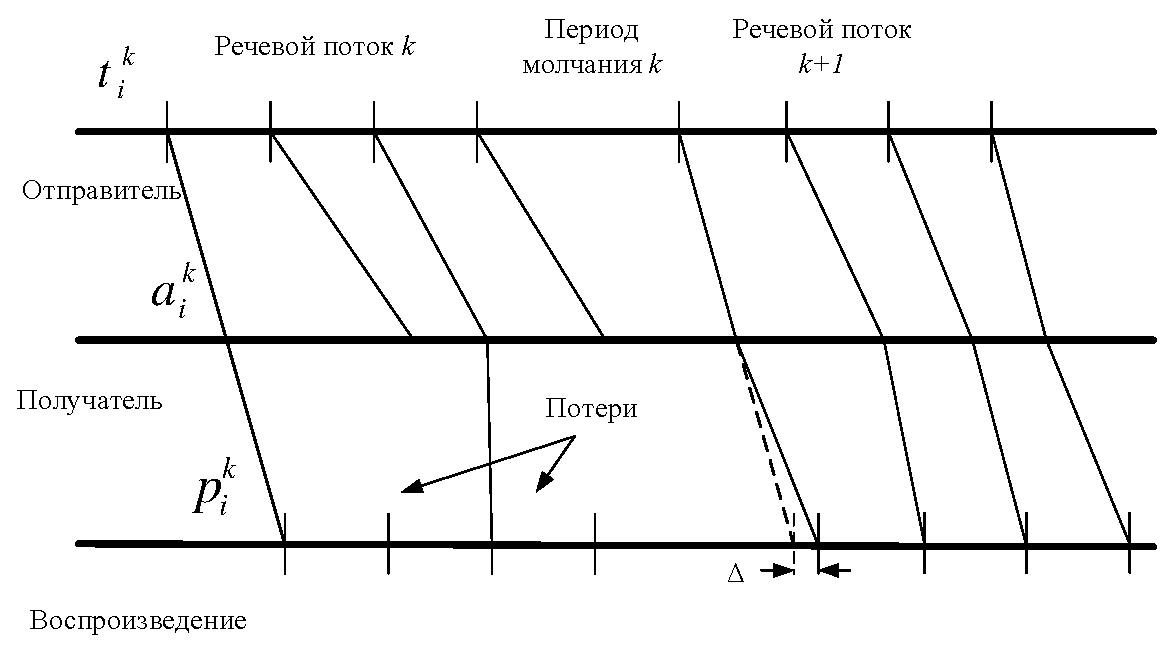
\includegraphics[width=1\linewidth]{3chapter/4b.eps} б) \\
\end{minipage}
\captionsetup{format=myformat,indention=2cm}
\caption{Схема регулировки задержки воспроизведения в паузах между речевыми потоками \\  а) с синхронной подстройкой \\б) с подстройкой первого пакета речевого потока }
\label{img3:manageDelay}
\end{figure}


Синхронизированный способ сводит к минимуму потери пакетов, но влияет на длину исходного речевого потока, что приводит к проблемам с разборчивостью восстановленной речи. По этой причине разрабатываемый буфер компенсации джиттера будет основан на алгоритме с подстройкой задержки только в периоды молчания.


\section{Анализ существующих алгоритмов компенсации джиттера.} \label{sect3_4}
\subsection{Алгоритм фиксированного буфера компенсации джиттера.} \label{sect3_4_1}

Наиболее простой и эффективной моделью отбрасывания пакетов является фиксированный буфер компенсации джиттера, который обозначает, как отбрасываемые, все пакеты, задержка которых больше чем минимальная задержка передачи потока пакетов плюс фиксированная длина буфера для сглаживания джиттера.
Рассмотрим пример алгоритма от сетевого до прикладного уровня, предполагая, что на терминале получателя используется буфер компенсации джиттера с фиксированной длиной:
\begin{enumerate}
\item Отметить как потерянные все пакеты с неверной контрольной суммой UDP.
\item Отметить как отбрасываемые все пакеты, задержка которых больше, чем минимальная задержка передачи потока пакетов плюс (фиксированная) длина буфера для сглаживания джиттера, или задержка которых меньше чем установленный минимум. 
\item Суммировать среднюю задержку в сети со средней задержкой терминала источника и терминала получателя, чтобы получить общую среднюю задержку, или суммировать минимальную задержку в терминале источника и минимальную задержку в сети с максимальной задержкой терминала получателя (отражающую максимальное время использования буфера для сглаживания джиттера).
\end{enumerate}

В вышеприведенном шаге 2 минимальную задержку передачи следует оценивать на коротких интервалах, например 10 секунд. Данное минимальное значение первого интервала используется всегда, не считая краткосрочного увеличения минимума вне диапазона адаптации буфера. В этом случае ни один из пакетов не будет доставлен на верхние уровни и буфер компенсации джиттера должен быть переустановлен на новый минимум, что вероятно будет происходить на практике. Или же, если краткосрочное значение минимума уменьшиться до величины, при которой высокий процент (временно 50\%) пакетов были бы помечены как потерянные из-за раннего поступления, то буфер компенсации джиттера должен быть переустановлен на новый минимум.

\subsection{Алгоритм адаптивного буфера компенсации джиттера.} \label{sect3_4_2}

Фиксированный буфер компенсации джиттера может быть заменен эмуляцией адаптивного буфера компенсации джиттера, как описано в данном пункте, когда имеется информация о временной последовательности потока пакетов. 
Временные последовательности поступления пакетов могут быть использованы эмулятором адаптивного буфера компенсации джиттера при определении динамики размера буфера и среднего времени использования буфера (задержка) для этой последовательности. Эта средняя задержка может быть объединена с другими константами задержки в терминале получателя для получения оценки средней задержки в терминале получателя. 
Рассмотрим пример эмулятора адаптивного буфера для сглаживания джиттера с коррекцией задержки в промежутках молчания \cite{Ramjee}. Чтобы определить время воспроизведения для пакета $k$-ого, мы рассмотрим два случая, в зависимости от того является $k$-ый пакет первым в речевом потоке или нет:
Если $k$-ый пакет является первым в речевом потоке $i$, то его время воспроизведения рассчитывается как:

\begin{equation}\label{eq3:playout}
p(k)=t(k)+\hat{x}(k)+\gamma\cdot\hat{\nu}(k),
\end{equation}

\noindent где $\hat{x}(k)$ - оценка среднего значения сквозной задержки, $\hat{\nu}(k)$ - оценка отклонения от среднего значения сквозной сетевой задержки, $\gamma$ - константа, используемая для установки времени воспроизведения так чтобы только небольшая часть поступающих пакетов была потеряна \cite{Ramjee}. Эта константа равна 4 во всех экспериментах, выполняемых в \cite{Ramjee}. В \cite{Moon} это значение варьируют от 1 до 20, что бы добиться различного процента потерь. Чтобы пересчитать среднюю сетевую задержку и его отклонение, используются следующие уравнения:

\begin{equation}\label{eq3:playout_d}
\hat{x}^{i}(k)=\alpha\cdot\hat{x}^{i}(k-1)+(1-\alpha)\cdot x^{i}(k),
\end{equation}

\begin{equation}\label{eq3:playout_v}
\hat{\nu}^{i}(k)=\alpha\cdot\hat{\nu}^{i}(k-1)+(1-\alpha)\cdot | \hat{x}^{i}(k)-x^{i}(k) |.
\end{equation}

Эти уравнения представляю собой линейные рекурсивные фильтры, где коэффициент $\alpha$ называется шаговой постоянной, $\alpha\leq1$ и обеспечивает устойчивость процедуры. В работе \cite{Ramjee} значение $\alpha$ выбрано равным 0.98002. 

Очевидно, что эти уравнения являются преобразованными уравнениями стохастической аппроксимации типа Роббинса-Монро и получаемая оценка $\hat{x}^{i}(k)$ и $\hat{\nu}^{i}(k)$, является оптимальной для оценивания случайной величины для которых уравнение состояния $x(k)=x(k-1)$. 
В нашем случае сетевая задержка представляет случайный процесс, поэтому оценки (\ref{eq3:playout_d}), (\ref{eq3:playout_v}) позволяют получить лишь средние значения задержек. 
Нас же интересуют их текущие значения. Адекватной процедурой для оценки текущих параметров случайного процесса является процедура Калмана-Бьюси.




\section{Постановка научной задачи и формулировка частных задач исследования } \label{sect1_tasks}

Следовательно, актуальной является научная задача, которая состоит в разработке предварительного буфера компенсатора джиттера на границе проводной и беспроводной сети способного компенсировать различные типы джиттера.
В ходе решения научной задачи сформулированы частные задачи исследования:
\begin{enumerate}
  \item Провести анализ статистических характеристик джиттера в стационарных и беспроводных сетях.
  \item Определить основные механизмы влияния на параметры джиттера.
  \item Определить статистические нестационарности джиттера и произвести классификацию нестационарных явлений задержки.
  \item Обосновать и разработать математическую модель джиттера, позволяющую отображать динамику изменений состояний.
  \item Разработать алгоритмы статистической оценки параметров джиттера и управления с целью его минимизации.
  \item Разработать практические предложения по выбору параметров и мест установки агента минимизации джиттера на границе стационарной и мобильной сети.
\end{enumerate}


\section{Выводы по первому разделу } \label{sect1_conclus}

\begin{enumerate}
\item Согласно прогнозам, к 2018 году мировой трафик данных увеличится в 12 раз. Данная тенденция обусловлена увеличением объемов доступного контента и ростом скорости передачи данных в мобильных сетях по мере развития технологий HSPA и LTE.
Сервисы с потоковым видео и аудио являются крупнейшим сегментом трафика в мобильных сетях благодаря значительному проникновению смартфонов на потребительский рынок:
если в 2012 году они составляли 40\% от общего объема продаж телефонов в мире, то только в первом квартале 2013 на долю смартфонов пришлось около половины продаж.
Вследствие чего исследования направленные на обеспечение требуемого качества обслуживания для мобильных абонентов являются актуальными.
\item Сети LTE с помощью технологии VoLTE, позволяют предоставлять услуги реального времени, 
такие как речевая связь в HD качестве, видео связь, организация конференций с эффектом присутствия и т. д., которые критичны к джиттеру задержки. 
Беспроводные сети LTE и проводные сети, через которые передаются пакеты этих услуг, могут быть подвержены различным факторам, которые увеличивают джиттер задержки. 
Поэтому предложено разработать метод компенсации джиттера на границе проводной и беспроводной сети, чтобы улучшить качество предоставления услуг реального времени в сетях LTE.

\item Проведен анализ требований QoS для предоставления сервисов реального времени.
Анализ показал, что основными факторами, влияющими на качество предоставления сервисов, являются задержка передачи, процент потерянных и поврежденных пакетов и джиттер задержки.
Сервисы реального времени с повышенной степенью взаимодействия критичны к джиттеру и задержке. Вследствие, чего необходимо решить проблему чрезмерно большого внесения задержки буфером компенсации джиттера. 
Предложено разработать адаптивный буфер компенсации джиттера, который бы учитывал текущее состояние сети, а также разработать способ его внедрения  в сети LTE.
\item Проанализирован принцип действия буфера компенсации джиттера. 
Показано, что буфер преобразовывает джиттер задержки в другие характеристики такие, как общая задержка и общие потери. 
Работа буфера является компромиссом между задержкой и потерями, который представлен в виде порога в диапазоне изменения задержки.
Также проведена систематизация основных принципов управления буфером компенсации джиттера. 
На основе анализа был выбран адаптивный принцип управления с подстройкой времени задержки первого пакета каждого речевого потока. 
Выбранный принцип основан на том, что дополнительная задержка буферизации вносится только в паузах между речевой активностью, что позволяет исключить влияние буфера на длину речевой активности.
В противном случае работа буфера могла бы привести к проблемам с разборчивостью речи.


\end{enumerate}

\clearpage




